\documentclass[12pt]{article}

% Add this line to use the geometry package
\usepackage[a4paper, margin=3.2cm]{geometry}
\usepackage[italian]{babel}
\usepackage[utf8]{inputenc}
\usepackage[T1]{fontenc}
\usepackage{listings}
\usepackage{xcolor} %color customization
\usepackage{colortbl} 

\input{style/common.tex}
\input{style/scala.tex}

\lstset{frame=, basicstyle={\footnotesize\ttfamily}}

\lstset{
    language=VHDL,               % Set language to VHDL
    basicstyle=\ttfamily,        % Set basic font style
    keywordstyle=\color{red},   % Keywords in blue
    identifierstyle=\color{blue}, % Identifiers in black
    commentstyle=\color{green},  % Comments in green
    stringstyle=\color{red},     % Strings in red
    stepnumber=1,                % Line number step (every line)
    numbersep=10pt,              % Space between line numbers and code
    backgroundcolor=\color[HTML]{e6e6e6}, % Light gray background
    frame=single,                % Frame around the code
    rulecolor=\color{black},     % Frame color
    breaklines=true,             % Automatic line breaking
    tabsize=2,                   % Tab size
    showstringspaces=false,      % Don't show spaces in strings
    captionpos=b,                % Caption position: bottom
    escapeinside={\%*}{*)}       % Escape to LaTeX with %* and *)
}

%BLZ DONT REMOVE THESE PACKAGES I NEED THEM FOR DRAWING THE FSM :-)
\usepackage{tikz}
\usepackage{float}
\usetikzlibrary{automata,positioning}
%THIS PACKAGE MAKE THE TEXT GO AROUND INSTEAD OF BREAK IT WITH THE "-" WHEN IT REACHS THE BORDER OF THE DOCS. 
\usepackage{microtype}

\usepackage{graphicx}
\usepackage{pdfcomment}
\graphicspath{ {images/} }

%-----------------------------------------BEGIN DOC----------------------------------------

\begin{document}

\title{{\Huge Prova Finale Reti Logiche{\large\linebreak\\}}{\Large Anno accademico 2023-2024 - Politecnico di Milano\linebreak\linebreak}}

\author{Samuele Grisoni\\
Codice Persona: 10810440\\
\\
Alessio Guarisco\\
Codice Persona: 10795876\\
}
\date{1 Settembre 2024}
\maketitle
\vspace{2cm}
\begin{center}
    
\includegraphics[width=0.6\linewidth]{images/Logo_Politecnico_Milano.png}
\end{center}

\newpage

%-----------------------------------------CONTENT-------------------------------------
\tableofcontents\label{c}
\newpage

%------------------------------------------TEXT--------------------------------------------

%--------------------------------------Introduzione--------------------------------------

\section{Introduzione} \label{Introduzione}%------------------------------
\subsection{Obiettivo}
L'obiettivo della seguente relazione è documentare l'architettura e lo sviluppo di un elemento hardware descritto in VHDL per l'elaborazione di una sequenza di numeri.
Lo scopo finale è completare la sequenza in maniera da ottenere una lista continua e discreta di valori. 
Il modulo hardware dovrà quindi interfacciarsi con una memoria da cui leggere la sequenza iniziale e scrivere al contempo la sequenza corretta. 
Nel nostro caso, lo stream è composto da un valore decimale, seguito da un valore di credibilità del numero appena letto. La credibilità rappresenta l'accuratezza del valore appena letto ed è un numero da 31 a 0.
Quando il valore numerico è nullo sarà necessario sostituire lo zero in memoria con l'ultimo valore numerico noto. Il valore di credibilità in questo caso verrà diminuito.

\subsubsection{Example}
Segue un esempio dell'esecuzione del programma con la seguente stringa di valori:
\textbf{128, 64, 0, 0, 0}


\begin{table}[h]
    \centering
    \begin{minipage}{0.45\textwidth}
        \centering
        
        % Please add the following required packages to your document preamble:
        % \usepackage[table,xcdraw]{xcolor}
        % Beamer presentation requires \usepackage{colortbl} instead of \usepackage[table,xcdraw]{xcolor}
        \begin{tabular}{cc}
        \rowcolor[HTML]{FFFFFF} 
        \textbf{Indirizzo}                                & \textbf{Valore}                                             \\ \hline
        \multicolumn{1}{|c}{...}                          & \multicolumn{1}{c|}{...}                                    \\
        \rowcolor[HTML]{E6E6E6} 
        \multicolumn{1}{|c}{\cellcolor[HTML]{E6E6E6}1234} & \multicolumn{1}{c|}{\cellcolor[HTML]{E6E6E6}10000000 (128)} \\
        \multicolumn{1}{|c}{1235}                         & \multicolumn{1}{c|}{00000000 (0)}                           \\
        \rowcolor[HTML]{E6E6E6} 
        \multicolumn{1}{|c}{\cellcolor[HTML]{E6E6E6}1236} & \multicolumn{1}{c|}{\cellcolor[HTML]{E6E6E6}01000000 (64)}  \\
        \multicolumn{1}{|c}{1237}                         & \multicolumn{1}{c|}{00000000 (0)}                           \\
        \rowcolor[HTML]{E6E6E6} 
        \multicolumn{1}{|c}{\cellcolor[HTML]{E6E6E6}1238} & \multicolumn{1}{c|}{\cellcolor[HTML]{E6E6E6}00000000 (0)}   \\
        \multicolumn{1}{|c}{1239}                         & \multicolumn{1}{c|}{00000000 (0)}                           \\
        \rowcolor[HTML]{E6E6E6} 
        \multicolumn{1}{|c}{\cellcolor[HTML]{E6E6E6}1240} & \multicolumn{1}{c|}{\cellcolor[HTML]{E6E6E6}00000000 (0)}   \\
        \multicolumn{1}{|c}{1241}                         & \multicolumn{1}{c|}{00000000 (0)}                           \\
        \rowcolor[HTML]{E6E6E6} 
        \multicolumn{1}{|c}{\cellcolor[HTML]{E6E6E6}1242} & \multicolumn{1}{c|}{\cellcolor[HTML]{E6E6E6}00000000 (0)}   \\
        \multicolumn{1}{|c}{1243}                         & \multicolumn{1}{c|}{00000000 (0)}                           \\
        \multicolumn{1}{|c}{...}                          & \multicolumn{1}{c|}{...}                                    \\ \hline                                    
        \end{tabular}

        \caption{Stato iniziale della memoria}
    \end{minipage}\hfill
    \begin{minipage}{0.45\textwidth}
        \centering
                \begin{tabular}{cc}
        \rowcolor[HTML]{FFFFFF} 
        \textbf{Indirizzo}                                & \textbf{Valore}                                             \\ \hline
        \multicolumn{1}{|c}{...}                          & \multicolumn{1}{c|}{...}                                    \\
        \rowcolor[HTML]{E6E6E6} 
        \multicolumn{1}{|c}{\cellcolor[HTML]{E6E6E6}1234} & \multicolumn{1}{c|}{\cellcolor[HTML]{E6E6E6}10000000 (128)} \\
        \multicolumn{1}{|c}{1235}                         & \multicolumn{1}{c|}{00011111 (31)}                           \\
        \rowcolor[HTML]{E6E6E6} 
        \multicolumn{1}{|c}{\cellcolor[HTML]{E6E6E6}1236} & \multicolumn{1}{c|}{\cellcolor[HTML]{E6E6E6}01000000 (64)}  \\
        \multicolumn{1}{|c}{1237}                         & \multicolumn{1}{c|}{00011111 (31)}                           \\
        \rowcolor[HTML]{E6E6E6} 
        \multicolumn{1}{|c}{\cellcolor[HTML]{E6E6E6}1238} & \multicolumn{1}{c|}{\cellcolor[HTML]{E6E6E6}01000000 (64)}   \\
        \multicolumn{1}{|c}{1239}                         & \multicolumn{1}{c|}{00011110 (30)}                           \\
        \rowcolor[HTML]{E6E6E6} 
        \multicolumn{1}{|c}{\cellcolor[HTML]{E6E6E6}1240} & \multicolumn{1}{c|}{\cellcolor[HTML]{E6E6E6}01000000 (64)}   \\
        \multicolumn{1}{|c}{1241}                         & \multicolumn{1}{c|}{00011101 (29)}                           \\
        \rowcolor[HTML]{E6E6E6} 
        \multicolumn{1}{|c}{\cellcolor[HTML]{E6E6E6}1242} & \multicolumn{1}{c|}{\cellcolor[HTML]{E6E6E6}01000000 (64)}   \\
        \multicolumn{1}{|c}{1243}                         & \multicolumn{1}{c|}{00011100 (28)}                           \\
        \multicolumn{1}{|c}{...}                          & \multicolumn{1}{c|}{...}                                    \\ \hline                                     
        \end{tabular}

        \caption{Stato della memoria dopo l'esecuzione}
    \end{minipage}
\end{table}


\subsection{Idea di Base}
Il processo è simile a quello utilizzato da alcuni algoritmi di ricostruzione dati a partire da una serie incompleta di bit, oppure al meccanismo di decompressione di un'immagine.
Ad esempio, la nota libreria di analisi dati di Python "Panda" offre un algoritmo di interpolazione chiamato "Forward Fill" che, come nel nostro caso, prende l'ultimo valore noto e lo propaga per riempire un dataset incompleto.
Algoritmi come il Run-Length Encoding comprimono le sequenze ripetitive di dati. Questo significa che se dovesse avvenire la decompressione dei dati, l'ultimo valore noto viene ripetuto per riempire tutti i valori mancanti.

\newpage
\subsection{Interfaccia del Progetto}
\begin{lstlisting}[caption={interfaccia di progetto}, label=lst:vhdl_example]
entity project_reti_logiche is
    port (
            i_clk : in std_logic;
            i_rst : in std_logic;
            i_start : in std_logic;
            i_add : in std_logic_vector(15 downto 0);
            i_k   : in std_logic_vector(9 downto 0);
            
            o_done : out std_logic;
            
            o_mem_addr : out std_logic_vector(15 downto 0);
            i_mem_data : in  std_logic_vector(7 downto 0);
            o_mem_data : out std_logic_vector(7 downto 0);
            o_mem_we   : out std_logic;
            o_mem_en   : out std_logic
    );
end project_reti_logiche;
\end{lstlisting}

\subsection{Descrizione delle Porte}
\label{PortDescription}
\begin{itemize}
    \item \textbf{i\_clk:} clock in ingresso, generato dal Test Bench per sincronizzare il funzionamento della macchina.
    \item \textbf{i\_rst:} segnale asincrono di reset in ingresso, anch'esso generato dal Test Bench. Se 1 prepara il componente per ricevere il segnale di start.
    \item \textbf{i\_start:} Segnale di start in ingresso, generato dal Test Bench. Questo segnale avvia la sequenza di elaborazione.
    \item \textbf{i\_add:} vettore che rappresenta l'indirizzo di memoria da cui la sequenza da elaborare parte, generato dal Test Bench.
    \item \textbf{i\_k:} rappresenta la lunghezza della sequenza da elaborare, anch'esso generato dal Test Bench.
    \item \textbf{o\_done:} Segnale di uscita. Indica il completamento dell'elaborazione. Generato per comunicare al Test Bench che la sequenza è stata completamente processata.
    \item \textbf{o\_mem\_address} Vettore di uscita che contiene l'indirizzo della memoria da cui leggere o scrivere i dati.
    \item \textbf{i\_mem\_data:} Vettore di ingresso che trasporta i dati letti dalla memoria in corrispondenza dell'indirizzo fornito.
    \item \textbf{o\_mem\_data:} Vettore di uscita che invia i dati da scrivere nella memoria all'indirizzo specificato.
    \item \textbf{o\_mem\_en:} Segnale di uscita che funge da abilitazione per l'accesso alla memoria. Questo segnale deve essere alto (=1) per consentire l'operazione di lettura o scrittura.
    \item \textbf{o\_mem\_we:} Segnale di uscita che indica se l'operazione in corso è una scrittura. Deve essere alto (=1) per scrivere nella memoria; altrimenti, l'operazione predefinita è la lettura.
\end{itemize}
%----------------------------------ARCHITETTURA------------------------------------------

\newpage
\section{Architettura}
\subsection{La macchina a stati finiti}
\begin{figure} [H]
  \centering
  \begin{tikzpicture}[->, shorten >=1pt, auto, node distance=5cm, thick]
  
    \tikzstyle{every state}=[fill=gray!20, draw=black, text=black]

    \node[state, initial] (SETUPSTART) {SETUPSTART};
    \node[state] (IDLE) [right of=SETUPSTART] {IDLE};
    \node[state] (FIRSTREADWRITE) [below of=IDLE] {FIRSTREADWRITE};
    \node[state] (PRINTCREDIBILITY) [right of=FIRSTREADWRITE] {PRINTCREDIBILITY};
    \node[state] (SETUPINPUT) [below left of=FIRSTREADWRITE] {SETUPINPUT};
    \node[state] (INPUT) [right=5cm of IDLE] {INPUT};
    \node[state, accepting] (ENDSTATE) [above of=IDLE] {ENDSTATE};

    \path (SETUPSTART) edge [bend left] node {i\_k = 0} (ENDSTATE)
                      edge node {i\_k $\neq$ 0} (IDLE);
    \path (IDLE) edge [bend left] node {p\_s = SETUPSTART} (FIRSTREADWRITE)
                edge node {p\_s = SETUPINPUT} (INPUT);
    \path (FIRSTREADWRITE) edge node {} (PRINTCREDIBILITY);
    \path (PRINTCREDIBILITY) edge [bend left] node {} (SETUPINPUT);
    \path (SETUPINPUT) edge [bend left] node {} (IDLE);
    \path (INPUT) edge [bend right, pos=0.25] node [left] {counter $>$ 2 $\times$ (i\_k - 1)} (ENDSTATE)
                 edge node {else} (PRINTCREDIBILITY);

  \end{tikzpicture}
  \caption{\label{fig:fsm}Schema della FSM realizzata}
\end{figure}

La figura \ref{fig:fsm} rappresenta uno schema semplificato della FSM utilizzata per risolvere il problema dato. La semplificazione, rispetto al codice fornito, è stata effettuata per meri motivi grafici e riguarda nome e contenuto di alcune variabili. Sono state inoltre rimosse alcune transizioni che, seppur presenti nel codice, risulta impossibile che si verifichino. In particolare nel nostro componente è presente una variabile "previous\_state" che tiene traccia dello stato visitato prima del nodo IDLE. Tale variabile è stata trascritta come \textit{ p\_s} all'interno dello schema. \\
È inoltre importante notare come \textit{i\_k} nello schema è stato rappresentato come un segnale formato da un singolo bit, quando esso è in realtà formato da un vettore di 10 bit.\\

Lo stato di partenza della FSM è rappresentato dallo stato di \textbf{SETUPSTART}, il quale si occupa di abilitare la memoria impostando \textit{o\_mem\_en = 1}, impostare la variabile di conteggio \textit{counter = 0} e di effettuare un controllo sul numero di parole da leggere, \textit{i\_k}. Se tale segnale è uguale a zero imposta lo stato corrente a ENDSTATE in modo da terminare l'esecuzione del componente al prossimo ciclo di clock. Nel caso in cui il numero di parole sia diverso da zero, SETUPSTART imposta la memoria in modalità di lettura mettendo \textit{i\_mem\_we} a \textit{0}, legge la prima parola presente sull'indirizzo in ingresso \textit{i\_add} e imposta il prossimo stato a IDLE.\\

Lo stato di \textbf{IDLE} è introdotto, per compensare la lentezza di risposta nella memoria in seguito a una richiesta di lettura. In particolar modo se lo stato precedentemente visitato è SETUPSTART imposta la variabile \textit{current\_state} a FIRSTREADWRITE; altrimenti, se lo stato visitato in precedenza è SETUPINPUT, imposta tale variabile a INPUT. \\

Lo stato di \textbf{FIRSTREADWRITE} si occupa della lettura della prima parola in input. Se tale parola è \textit{0} presenta un edge-case, richiedendo di impostare la credibilità a 0; altrimenti essa viene impostata a 31, come da specifica. Lo stato si occupa inoltre di impostare la memoria in modalità scrittura in modo da poter stampare la credibilità al prossimo ciclo di clock.\\

\textbf{PRINTCREDIBILITY} è lo stato che si occupa di stampare la credibilità nella cella di memoria posta all'indirizzo ottenuto come \textit{i\_add + contatore + 1}.\\

Lo stato di \textbf{SETUPINPUT} imposta i corretti segnali per la lettura della prossima parola dalla memoria. In particolare la memoria viene messa in lettura, la variabile counter viene aumentata di 2, in modo da poter leggere la parola successiva, e il nuovo indirizzo di memoria da leggere, \textit{o\_mem\_addr}, viene aggiornato con la somma di \textit{i\_add + counter}.\\

Lo stato di \textbf{INPUT} si occupa di verificare se sono state lette \textit{i\_k} parole confrontando tale segnale con la variabile counter o, in alternativa, di aggiornare la credibilità in base alla nuova parola letta. 
Quando counter viene confrontato con \textit{i\_k} è necessario moltiplicare tale segnale per 2 affinchè la disequazione risulti corretta. Se tale espressione risulta verificata, la variabile \textit{current\_state} viene impostata pari a ENDSTATE in modo da terminare il processo al prossimo ciclo di clock. Se la disequazione non è vera, è necessario leggere almeno un'altra parola e aggiornare la variabile \textit{credibility} di conseguenza. Se la parola letta risulta essere 0 allora la credibilità viene scalata di 1, purchè sia positiva, come da specifica; altrimenti viene impostata al valore 31. Viene impostata la variabile \textit{current\_state} a PRINTCREDIBILITY in modo da poter scrivere in memoria la credibilità al prossimo ciclo di clock.\\

Lo stato di \textbf{ENDSTATE} disabilita la memoria impostando \textit{o\_mem\_en} a 0 e segnala al TestBench di aver terminato il processo impostando il segnale \textit{o\_done} a \textit{1}. \\

\subsection{Lettura e scrittura in un singolo ciclo}
\label{SingleReading}
Il problema principale riscontrato durante lo sviluppo è stato la lentezza della memoria presente nel TestBench. Tale componente infatti introduce un ritardo di 1 ns che impedisce di scrivere la credibilità e leggere la parola successiva in due cicli di clock successivi come visibile nella figura \ref{fig:DisallignmentScreen}. \\
Come scritto in precedenza sia lo stato SETUPINPUT che lo stato di SETUPSTART hanno tra i vari loro compiti quello di impostare il corretto valore ai segnali per predisporre la memoria per la lettura. La risposta della TestBench a tale modifica non è però sicronizzata con la salita del segnale di clock, a causa del ritardo sopracitato, e una eventuale lettura eseguita nello stato immediatamente successivo a quest'ultimo comporta l'acquisizione di un input uguale a 0 nel caso di lettura immediatamente dopo SETUPSTART, o del valore della credibilty appena scritto nel caso di lettura dopo PRINTCREDIBILIY.\\
La soluzione a cui abbiamo pensato è stata quella di introdurre un insieme di \textit{SETUPSTATE} con il compito di fare da cuscinetto tra la scrittura e la lettura, impiegando un ciclo di clock, permettendo alla memoria di mostrare in uscita la parola corretta durante l'esecuzione di tale stato. Ciò permette di poter leggere il dato corretto nel ciclo di clock successivo. Tale soluzione è stata poi ottimizzata nello stato IDLE con l'obbiettivo di diminuire il numero di stati ridondanti.
\subsection{Scelte implementative nello sviluppo della FSM}
Per realizzare il componente sono state effettuate una serie di scelte implementatitive; alcune sono visibili nello schema \ref{fig:fsm} mentre altre sono state omesse per semplicità grafica.\\
Tra queste modifiche troviamo la scelta di gestire lo stato di IDLE con uno switch-case, di fatto realizzando una piccola FSM dentro la nostra macchina a stati. Quando si utilizza tale operatore, il linguaggio VHDL richiede che ogni possibile valore che può essere assunto dalla variabile presa in cosiderazione, sia gestito. Ciò ci ha costretti a creare un branch "others" che fa terminare il programma nel caso in cui \textit{previous\_state} abbia un valore diverso da SETUPINPUT o SETUPSTART. L'aggiunta di "others" fa in modo di evitare l'insorgere di latch nel nostro compoente, nonostante questa opzione non sia di fatto mai eseguita nel nostro codice. Questa scelta crea una possibile transazione tra IDLE e ENDSTATE ma tale collegamento, non essendo mai utilizzato, non è stato rappresentato nello schema della FSM.\\

Durante lo sviluppo si è preferito di rimanere in uno specifico stato per un solo ciclo di clock. Questa scelta è stata fatta per separare, da un punto di vista logico le operazioni effettuate dal nostro componente sulla memoria. Questa scelta si è rivelata molto elegante per rappresentare la FSM in quanto per determinati stati come INPUT, PRINTCREDIBILITY e IDLE il solo nome è sufficente a far capire il loro ruolo. Inoltre, poichè ogni stato effettua poche operazioni elementari, il codice scritto per ognuno di essi risulta corto, facilmente consultabile e modificabile.\\

Questa scelta implementativa ha reso necessario aumentare il numero di stati pur di non avere autoanelli e di conseguenza avere sequenze di stati che, in teoria, potevano essere unite. Un esempio di tale sequenza è formato da FIRSTREADWRITE-PRINTCREDIBILITY-SETUPINPUT. 
Si noti che l'introduzione di questi stati non rallenta l'esecuzione del nostro componente in quanto, come spiegato nella sezione \textit{\ref{SingleReading}}, sono comunque necessari 3 cicli di clock per completare una lettura e scrittura.\\

Un'ulteriore scelta implementativa, non rappresentata nel disegno della FSM, riguarda lo stato finale. In ENDSTATE, poichè non viene più aggiornata la variabile \textit{current\_state} ad ogni ciclo di clock, si ha un autoanello che riporta continuamente la FSM in ENDSTATE.

\subsection{Altri errori riscontrati durante lo sviluppo della FSM}
Durante la realizzazione della macchina a stati sopraindicata (\ref{fig:fsm}) sono stati riscontrati una serie di problemi minori, tra i più significativi troviamo:
\begin{itemize}
    \item \textbf{mem\_en\(\ne\) 0:} Nella prima iterazione della macchina, una volta raggiunto ENDSTATE, l'unica operazione effettuata era quella di impostare il segnale \textit{o\_done} a 1. Questo provocava un errore poichè la memoria era lasciata attiva, comportando un fallimento del test. La modifica, è stata quella di attribuire a ENDSTATE il compito di porre \textit{o\_mem\_en = 0} prima di eseguire qualsiasi altra istruzione.
    \item \textbf{Counter Overflow:} Durante l'esecuzione di TestBench con una grande quantità di parole, abbiamo incrontrato un overflow della variabile counter, utilizzata come offeset rispetto a \textit{i\_add} per calcolare le posizioni in cui scrivere la credibilty o leggere le nuove parole. Tale variabile era stata dimensionata a 10 bit come \textit{i\_k}, ovvero il segnale in ingresso che indica il numero di parole da leggere.\\
    Tale dimensionamento è risultato errato poichè counter aumenta di 1 per ogni parola da leggere e per ogni credibility da scrivere. Il risultato è quindi grande almeno il doppio rispetto al numero contenuto in \textit{i\_k}. Per risolvere questo problema è stato deciso di dimensionare counter a 16 bit, la dimensione di \textit{i\_add}.
\end{itemize}
\newpage

\section{Risultati Sperimentali}\label{Risultati Sperimentali}
\subsection{Sintesi}
\begin{figure}[h]
    \centering
    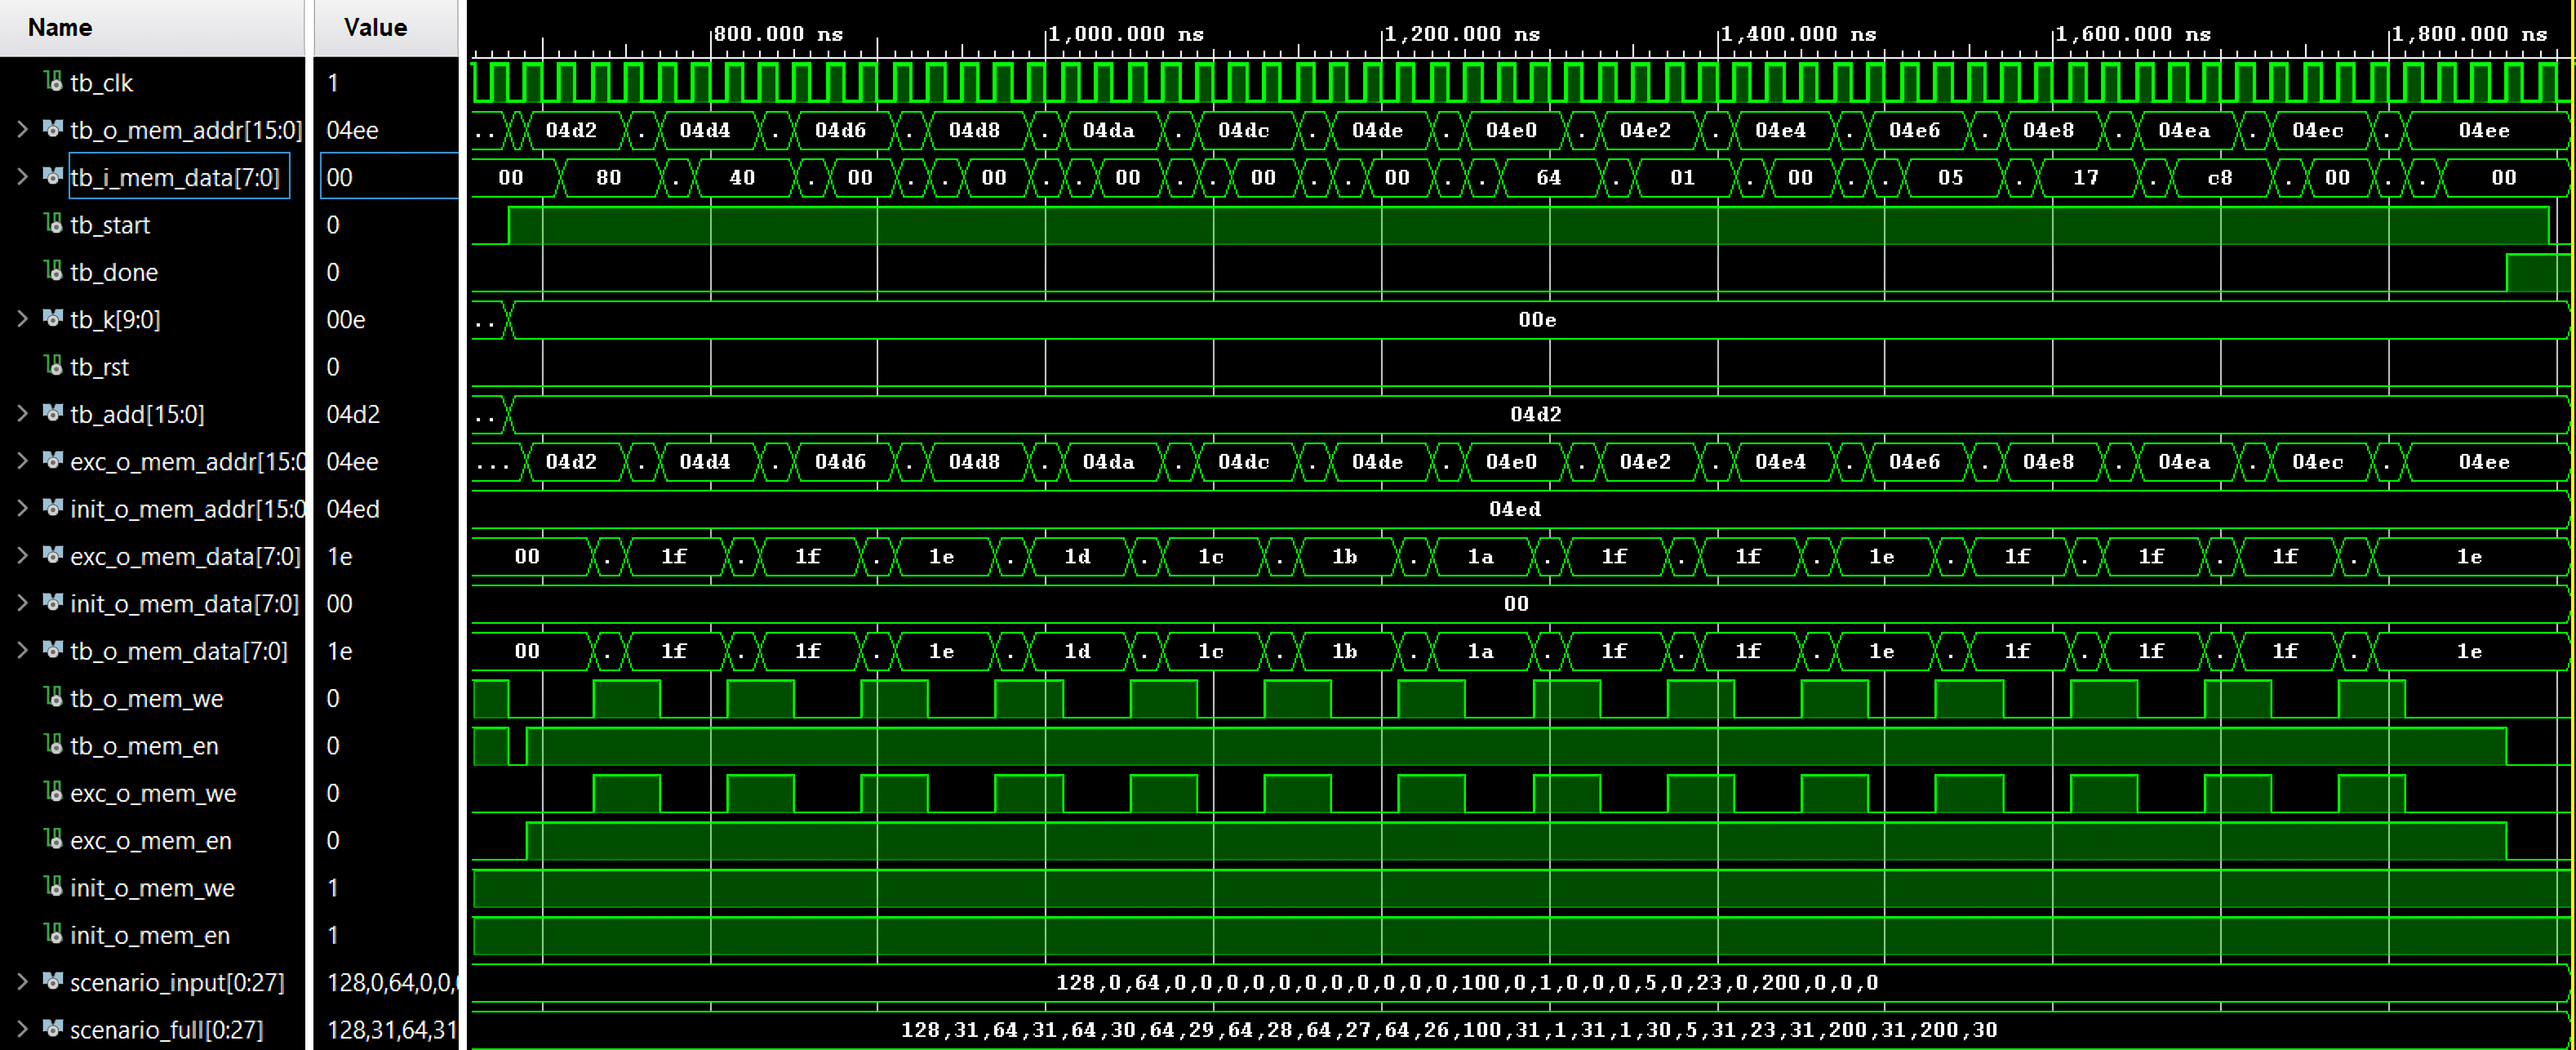
\includegraphics[width=\linewidth]{images/CompleteGraphs.png}
    \caption{Sintesi componente con TestBench ufficiale}
    \label{fig:SaliceTestBench}
\end{figure}
L'immagine mostra il risultato della sintesi del nostro componente. Poichè i segnali di ingresso e uscita del componente sono già stati descritti nella apposita sezione \ref{PortDescription} qui verranno analizzati, in ordine, solo i più rilevanti:
\renewcommand{\labelenumi}{\Roman{enumi}.}
\begin{enumerate}
    \item \textbf{tb\_clk:} Rappresenta il segnale di clock della TestBench.
    \item \textbf{exc\_o\_mem\_addr:} Rappresenta l'indirizzo a cui si sta effetuando l'operazione di scrittura o lettura nella TestBench. I numeri scritti dentro al segnale rappresentano, in HEX, il valore dell'indirizzo. Per motivi grafici sono stati omessi gli indirizzi in cui è stata scritta la credibilità, i quali però sono successivi agli indirizzi di lettura.
    \item  \textbf{tb\_i\_mem\_data:} Rappresenta il valore che si sta leggendo dall'indirizzo \textit{o\_mem\_add}. Già da questa immagine si può notare come esista un disallineamento tra l'aggiornamento del clock e dell'indirizzo di memoria rispetto all'aggiornamento del valore letto. 
    \item \textbf{tb\_start}: Rappresenta il segnale inviato dalla TestBench al nostro componente per avviare il processo. Si noti che questo segnale, come da specifica, rimane alto finchè il componente non dichiara di aver terminato il processo con alzando il segnale di \textit{tb\_done}.
    \item \textbf{tb\_done:} Si alza a 1 solo quando il processo è terminato. 
    \item \textbf{tb\_k:} Rappresenta la quantità di parole da dover leggere in HEX. In questa TestBench: 000e (14 in decimale).
\end{enumerate}
\newpage
\subsection{Aggiornamento memoria in ritardo}

\begin{figure}[h]
    \centering
    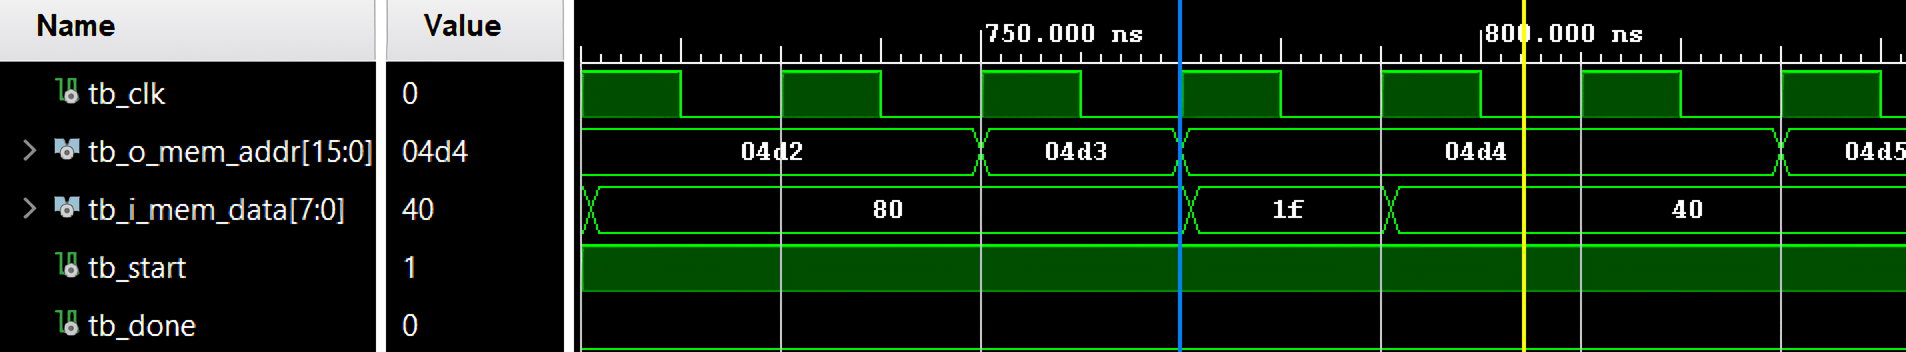
\includegraphics[width=\linewidth]{images/DisAlligmentGraph.png}
    \caption{Dettaglio di sintesi del TestBench ufficiale}
    \label{fig:DisallignmentScreen}
\end{figure}
In questa figura si evince chiaramente il problema indotto dal ritardo della memoria. In particolare ricordiamo che: il primo segnale rappresenta il clock, il secondo l'indirizzo della cella di memoria e il terzo il valore letto o scritto in tale cella. \\
Dal quarto ciclo di clock il componente si trova nello stato PRINTCREDIBILITY. Si può osservare come la scritta del valore di credibilità 1f (31  in decimale) avvenga dopo la salita del clock. Questo ritardo, sommato al ritardo indotto dall'operazione di lettura, impedisce di leggere il dato corretto contenuto nella cella 04d4 immediatamente dopo aver scritto nella cella 04d3. Effettuando la lettura al quinto ciclo di clock infatti andremmo a leggere il valore 1f, ovvero la credibility, invece della nuova parola 40 (64 in decimale).\\ 
Per risolvere tale problema è necessaro ritardare l'operazione di scrittura di un ciclo di clock e ciò avviene tramite lo stato IDLE. L'operazione di lettura avviene in corrispondenza della linea verticale gialla al sesto ciclo di clock. 

\vspace{0.5cm}


\subsection{Edge Cases}
\subsubsection{Estremi di K}
I casi limite per il valore di K sono K = 0 e K = 1023.


In particolare se K è pari a 0 non ci sono parole da elaborare.
Il modulo gestisce correttamente questa condizione senza entrare in loop o causare errori, e alzare immediatamente il segnale DONE.


Se K assume il valore massimo possibile (1023, dato che è un segnale a 10 bit)
Il modulo deve gestire correttamente l'intero intervallo di valori senza eccedere i limiti di memoria o causare overflow.
\newpage
\subsubsection{Sequenza di Zero}
\begin{figure}[h]
    \centering
    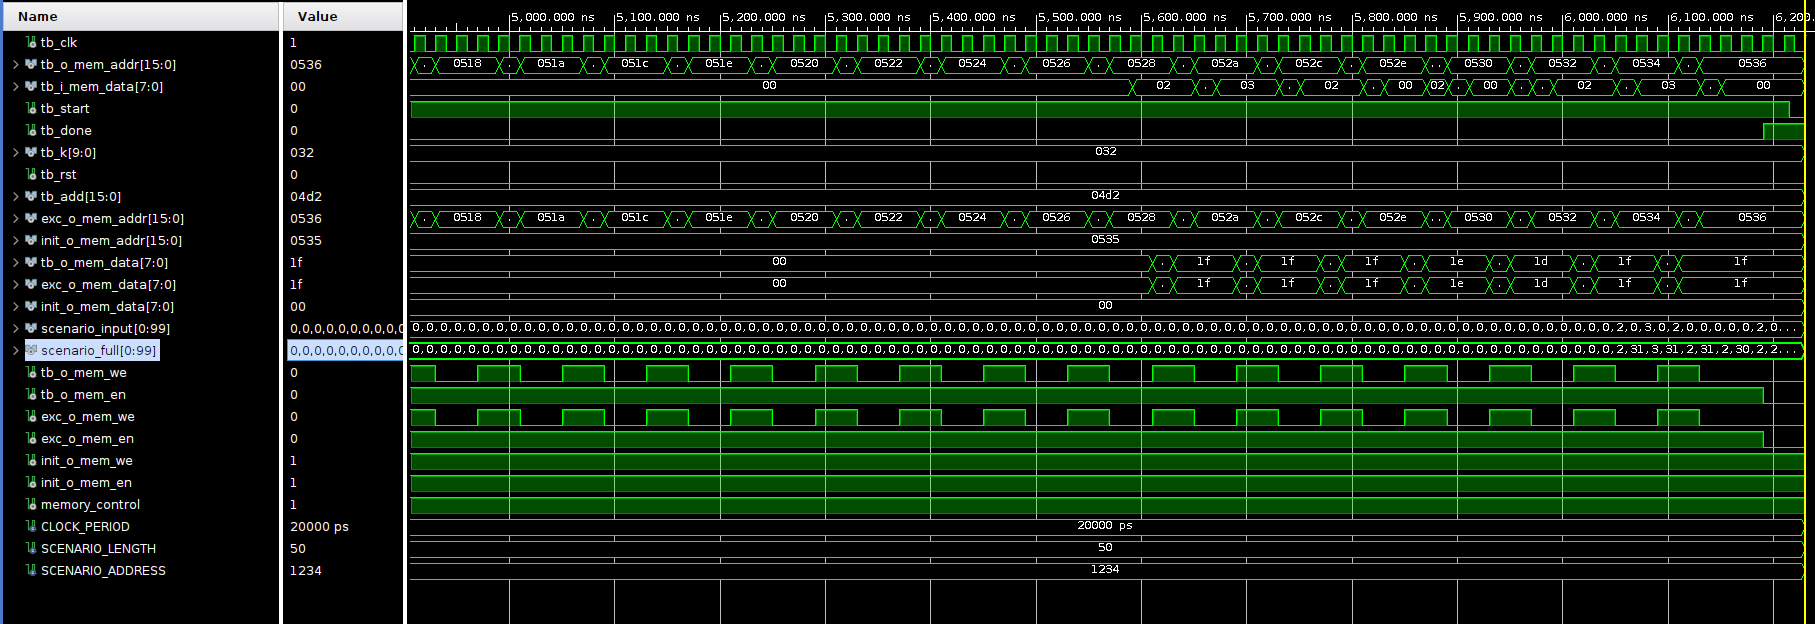
\includegraphics[width=\linewidth]{images/SerieZero.png}
    \label{fig:DisallignmentScreen}
\end{figure}

Si rilevano due casi limite legati alle sequenze di zero.

Il primo è una serie di più di 62 zeri. Questo fa sì che la credibility si azzeri ed è quindi possibile controllare che il modulo si comporti in maniera corretta, non andando in underflow ma mantenendo il valore della credibility a zero.

Il secondo caso è testato dalla testbench con una serie di numeri che iniziano con zero. Il comportamento osservato è mantenere gli zero all'interno della memoria, sia per la credibility sia per  il valore numerico.

Il modulo è stato fatto girare su una testbench che parte con una serie di valori numerici e credibilità zero, così da escludere comportamenti errati di entrambi i casi.


\subsubsection{Multipli Start}
\begin{figure}[h]
    \centering
    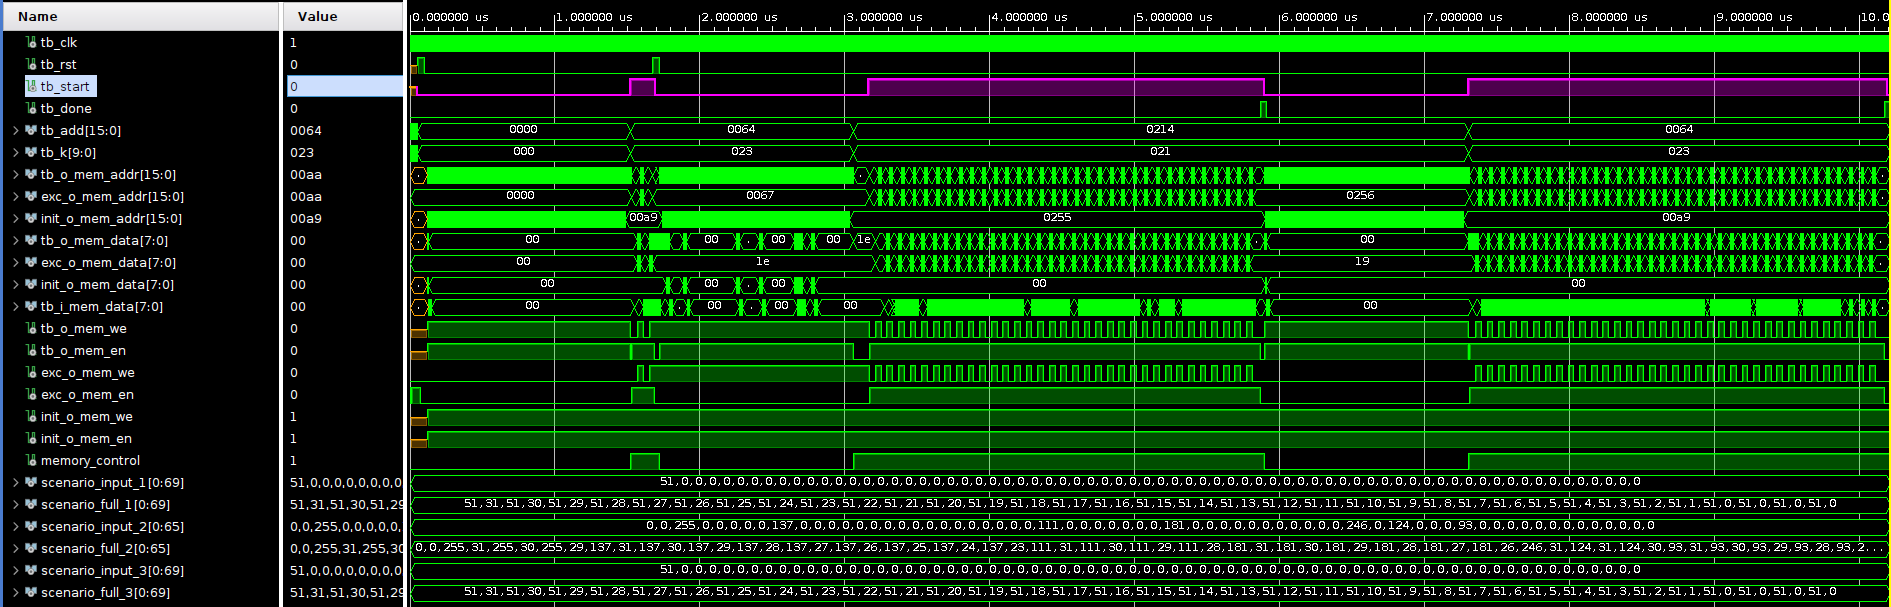
\includegraphics[width=\linewidth]{images/MoreStart.png}
    \label{fig:DisallignmentScreen}
\end{figure}
Dato che da specifica il modulo deve essere in grado di accettare un segnale START anche dopo che una serie numerica è terminata una testbench è stata utilizzata per testare la possibilità di avere più di uno START in una sola testbench.
\newpage
\subsubsection{Reset durante la lettura}
\begin{figure}[h]
    \centering
    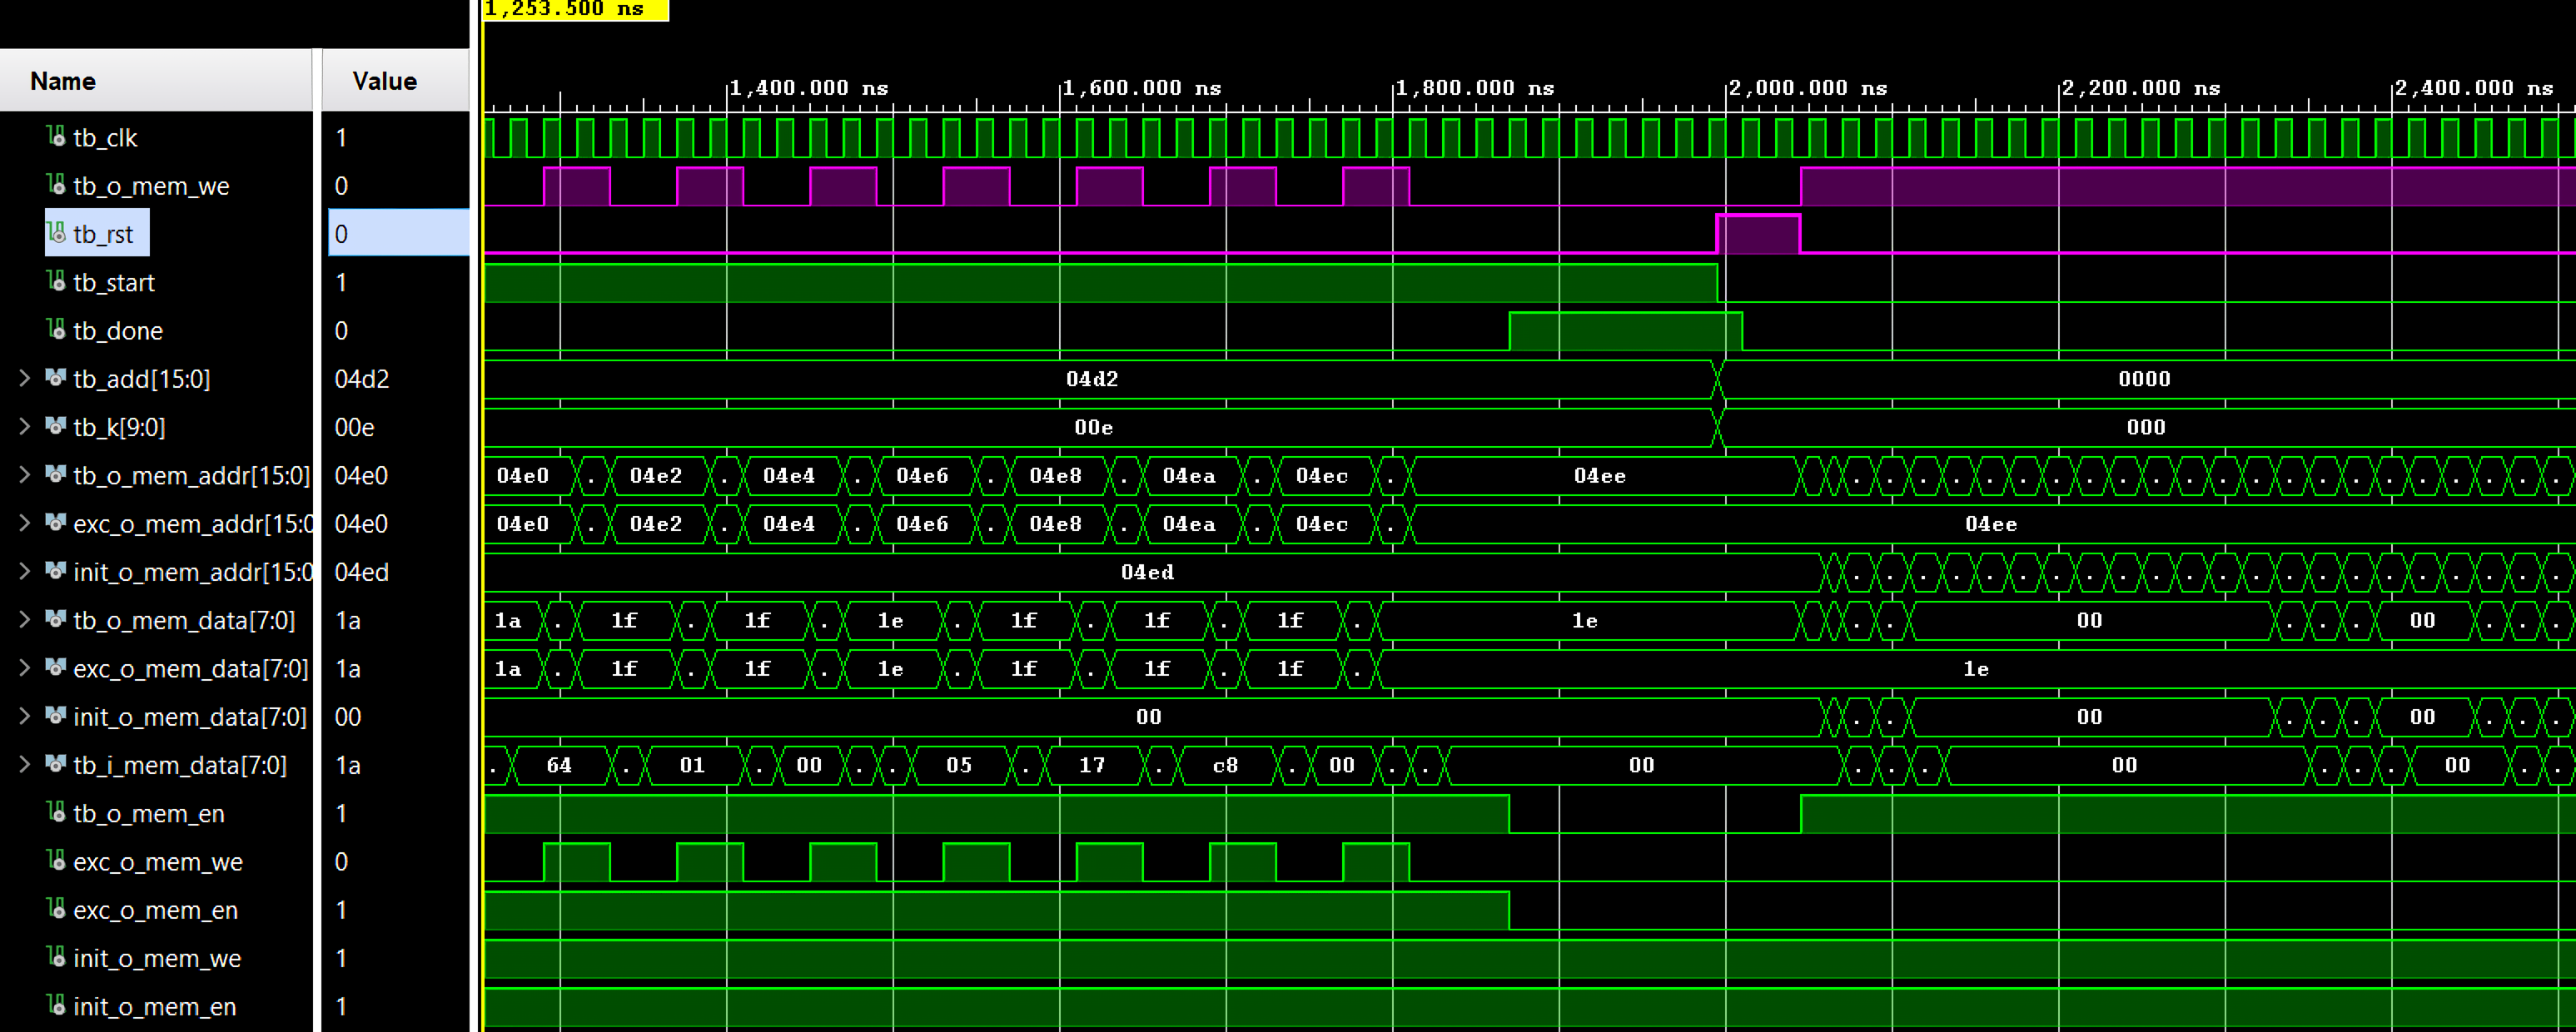
\includegraphics[width=\linewidth]{images/ResetRead.png}
    \label{fig:DisallignmentScreen}
\end{figure}
È stato esaminato il comportamento del modulo in presenza di un segnale di reset asincrono, attivato intenzionalmente durante una lettura dalla memoria. Questo test è cruciale per valutare la robustezza e l'affidabilità del modulo in situazioni in cui potrebbe verificarsi un reset imprevisto, interrompendo le operazioni in corso. È stato inoltre verificato che il modulo, dopo il reset, ritorna correttamente allo stato iniziale predefinito e rimane pronto per un successivo segnale di Start.

\subsubsection{Start durante il Reset}
\begin{figure}[h]
    \centering
    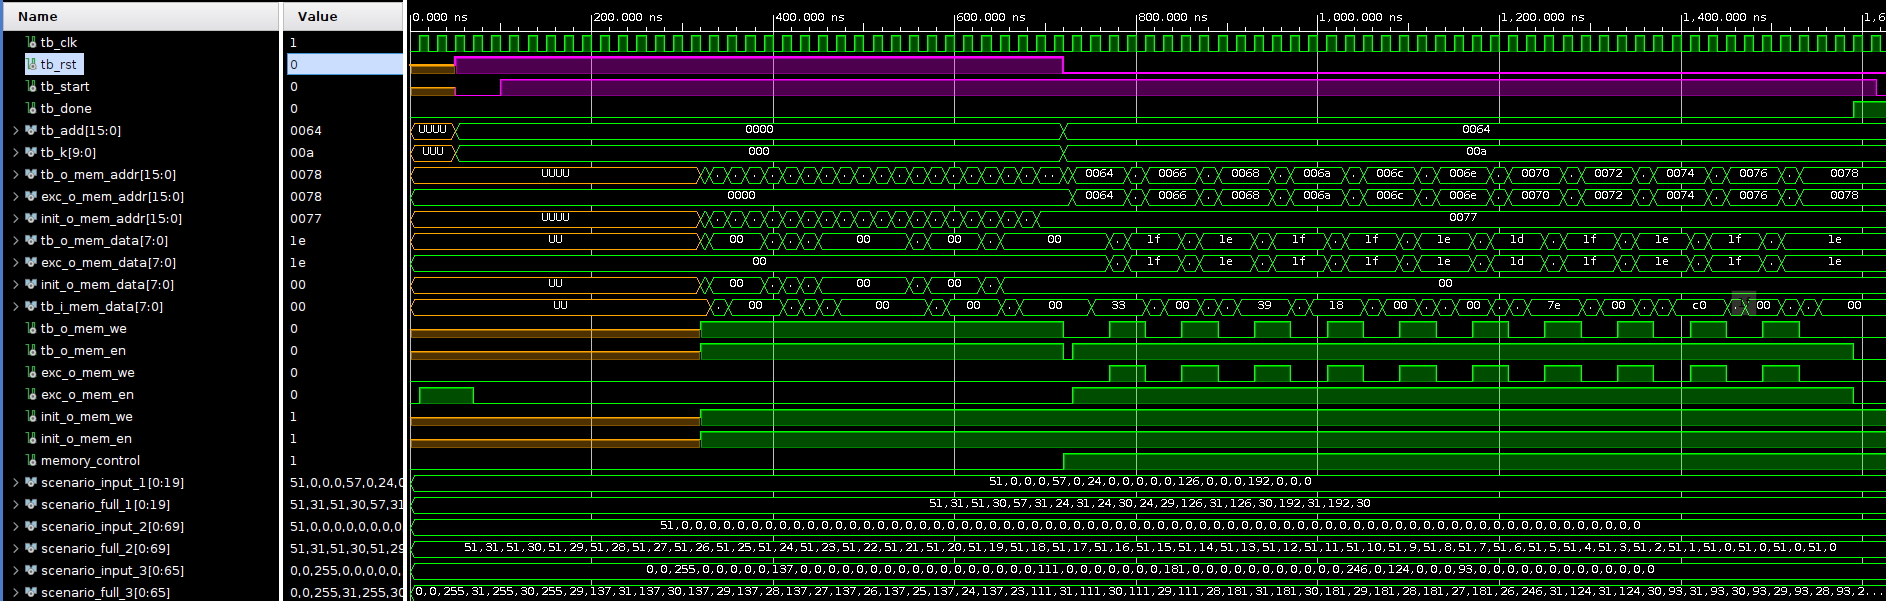
\includegraphics[width=\linewidth]{images/rstwhilestart.png}
    \label{fig:DisallignmentScreen}
\end{figure}
Un altro scenario critico testato è stato l'attivazione del segnale di Start mentre il modulo era soggetto a un segnale di Reset. Questo test è stato progettato per analizzare il comportamento del sistema in race condition tra il tentativo di avvio di una nuova operazione e la richiesta di ripristino allo stato iniziale. 

In particolare, è stato monitorato come il modulo gestisce la priorità tra questi due segnali, valutando se l'operazione di Start viene ignorata, ritardata, o se può innescare un comportamento anomalo. È stato inoltre verificato se il modulo, una volta completato il reset, è in grado di riconoscere correttamente il segnale di Start e avviare l'operazione desiderata senza errori. 

\newpage
\section{Conclusione}
Il progetto ha raggiunto l'obiettivo prefissato di sviluppare un modulo hardware in VHDL in grado di elaborare una sequenza di numeri, correggendo i valori mancanti attraverso la propagazione dell'ultimo valore noto. 

La scelta di scrivere il modulo in Behavioural per simulare un algoritmo informatico ci ha permesso di progettare in maniera funzionale una scheda Hardware che può essere utilizzata nel campo delle scienze informative.

Le scelte implementative adottate, come la suddivisione delle operazioni in stati distinti all'interno della macchina a stati finiti, si sono dimostrate efficaci nel gestire le complessità legate alla sincronizzazione della memoria e all'ottimizzazione dei tempi di esecuzione.

Nonostante si siano presentate alcune difficoltà iniziali, in particolare nella gestione dei ritardi della memoria, il progetto è stato completato con successo. Questo ha dimostrato la robustezza e l'efficienza della soluzione proposta, evidenziando l'importanza di un'attenta progettazione e implementazione nel contesto delle reti logiche.

 
\end{document}